%!TEX TX-program = xelatex
\documentclass[8pt]{article}
\usepackage{allan-eason}

\usetikzlibrary{positioning}
\usetikzlibrary{svg.path}

\graphicspath{ {./images/} }

\newcommand{\Date}{220413}
\newcommand{\Test}{三角与向量}

\newcommand{\Author}{Eason S.}
\newcommand{\Title}{\textcolor{allandarkblue}{\Date}\ \textcolor{allancyan}{\Test}\ 题目选解}

\author{\Author}
\title{\Title}
\date{}

\geometry{a4paper, scale=0.8}

\lhead{\Title}

\begin{document}

	\maketitle

	\athword{作者的话. } 这次测验还有点难度, 做得不好不要垂头丧气, 不要冲动, 不要愤怒. 认真总结教训, 积累经验, 学习方法.

	\section{填空题}
		\defword{1. }以下与\(\sin \left(\alpha - \dfrac{\pi}{2}\right)\)相等的有: (1) \(\sin \left(\dfrac{3\pi}{2} - \alpha \right)\), (2) \(\sin \left(\alpha + \dfrac{\pi}{2}\right)\), (3) \(\cos \left(\alpha + 15\pi\right)\). \answord{(1) (3)}.

		\answord{解析. }三角变换.
		~\\

		\defword{2. }设\(\tan \alpha = m (m \neq 0), \sin \alpha = \dfrac{m}{\sqrt{1+m^2}}\), 则\(\alpha\)可能为第\answord{一、四}象限角.

		\answord{解析. }三角变换.
		~\\

		\defword{3. }若\(\alpha \in \left(0, \dfrac{\pi}{2}\right)\), 则\(\log_{\cos \alpha} \left(1+\tan^2\alpha\right)=\ansmath{-2}\).

		\answord{解析. }三角变换.
		~\\

		\defword{4. }若扇形的弧长和面积均为\(4\), 则该扇形的弦心距长度为\answord{\(2\cos 1\)}.

		\answord{解析. }初中几何.
		~\\

		\defword{5. }函数\(y=2\tan \left(\dfrac{\pi}{6} - 3x\right)\)的单调\answord{减}(增/减)区间为\answord{\(\left(-\dfrac{\pi}{9} + \dfrac{k\pi}{3}, \dfrac{2\pi}{9} + \dfrac{k\pi}{3}\right), k \in \ZZ\)}.

		\answord{解析. }三角函数的单调性.

		\athword{答案不唯一.}
		~\\

		\defword{6. }若把函数\(y=\cos x-\sin x\)的图像做适当的变换后能得到\(y=\sqrt{2} \sin 2x\)的图像, 这样的移动可以是: 先将图像上所有点的横坐标\answord{除以\(2\)}, 再将图像向右平移\answord{\(\dfrac{3\pi}{8}\)}个单位.

		\answord{解析. }三角函数图像的变换; 三角变换.

		\athword{答案不唯一.}

		\athword{作者的话. }自己选的时候请先伸缩后平移, 反过来比较容易脑抽. 考虑实际平移情况的时候应当将平移量给予\(x, y\).
		~\\

		\defword{7. }将\(\cos \left(\alpha + \dfrac{\pi}{3}\right) \sin \left(\beta + \dfrac{\pi}{6}\right)\)化为和差的形式\answord{\(\dfrac{1}{2}\left[\cos\left(\beta + \alpha\right) + \sin \left(\beta - \alpha - \dfrac{\pi}{6}\right)\right]\)}.

		\answord{解析. }三角变换.

		\athword{答案不唯一.}
		~\\

		\defword{8. }若\(\abs{\vec{a} + \vec{b}}=3, \abs{\vec{a} - \vec{b}}=7\), 则\(\abs{\vec{a}}\)的取值范围是\answord{\([2, 5]\)}.

		\answord{解析. }向量的基本运算.

		\athword{作者的话. }此后所有出现的所谓“空间向量”“平面向量”等统一使用\(\vec{v}\)表示 (相对而言比较简洁明了), 仅在明确指明属于线性代数学科讨论范围 (e.g. 与矩阵进行运算) 时使用\(\vect{M}\)表示 (保持与矩阵运算样式的统一性). 物理文档中一般向量统一使用\(\vect{v}\)表示, 如遇到单位向量使用\(\hat{\vect{e}}\) (使用\(\hat{x}\)强调单位, \(\vect{x}\)强调向量).
		~\\

		\defword{9. }在\(\triangle ABC\)中, 记\(\ray{BA}=\vec{a}, \ray{BC}=\vec{b}\), 已知\(\abs{\vec{b}}=\sqrt{10}, \abs{\vec{a}+\vec{b}}=6, \abs{\vec{a}-\vec{b}}=4\), \(\ang{\vec{b}, \vec{a} - \vec{b}}=\ansmath{\arccos-\dfrac{\sqrt{10}}{8}}\) (用反三角表示).

		\answord{解析. }向量的基本运算.

		\calword{法一. }利用向量的基本运算的平行四边形法则进行计算/利用向量的和的模长推出向量的差的模长所在的边的中线进行计算.

		如图所示, 作向量\(\vec{a} + \vec{b}, \vec{a} - \vec{b}\), 令\(\ray{BD} = \vec{a} + \vec{b}, AC\)交\(BD\)于\(O\),

		\[
		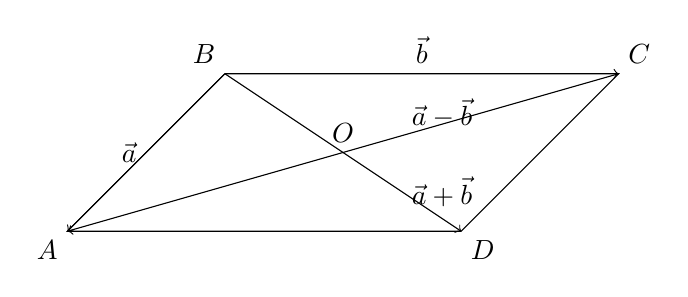
\begin{tikzpicture}[scale=1]
			\draw[black] (0, 0)--(5, 0)--(3, -2)--(-2, -2)--(0, 0) node at (0, 0) [anchor = south east]{\(B\)} node at (5, 0) [anchor = south west]{\(C\)} node at (3, -2) [anchor = north west]{\(D\)} node at (-2, -2) [anchor = north east]{\(A\)} node at (2.5, 0) [anchor = south]{\(\vec{b}\)} node at (-1, -1) [anchor = east]{\(\vec{a}\)};
			\draw[black, ->] (0, 0)--(3, -2) node at (2.25, -1.5) [anchor = west]{\(\vec{a} + \vec{b}\)};
			\draw[black, ->] (5, 0)--(-2, -2) node at (1.5, -1) [anchor = south]{\(O\)} node at (2.25, -0.5) [anchor = west]{\(\vec{a} - \vec{b}\)};
			\draw[black, ->] (0, 0)--(5, 0);
			\draw[black, ->] (0, 0)--(-2, -2);
		\end{tikzpicture}
		\]

		显然有

		\[
		\ang{\vec{b}, \vec{a} - \vec{b}} = \pi - \angle ACB.
		\]

		由于给出了\(BD, AC, AB, BC\)的长度以及平行四边形的对角线相互平分, 显然有\(OB=3, OC=2, BC=\sqrt{10}\), 由余弦定理可知\(\angle ACB = \arccos{\dfrac{\sqrt{10}}{8}}\), 则有\answord{\(\ang{\vec{b}, \vec{a} - \vec{b}} = \arccos{-\dfrac{\sqrt{10}}{8}}\)}.
		~\\

		\calword{法二. }利用向量的内积及相关量进行计算.

		由向量的内积运算, 显然有

		\[
		\vec{b} \cdot \left(\vec{a} - \vec{b}\right) = \abs{\vec{b}} \cdot \abs{\vec{a} - \vec{b}} \cdot \cos \ang{\vec{b}, \vec{a} - \vec{b}} = 4\sqrt{10} \cdot \cos \ang{\vec{b}, \vec{a} - \vec{b}} = \vec{a}\cdot\vec{b} - \abs{\vec{b}}^2 = \vec{a}\cdot\vec{b} - 10,
		\]
		\[
		\abs{\vec{a} + \vec{b}}^2 = \left(\vec{a} + \vec{b}\right)^2 = \vec{a}^2 + 2 \cdot \vec{a} \cdot \vec{b} + \vec{b}^2 = \abs{\vec{a}}^2 + 2 \cdot \vec{a} \cdot \vec{b} + \abs{\vec{b}}^2 =  \abs{\vec{a}}^2 + 2 \cdot \vec{a} \cdot \vec{b} + 10 = 36,
		\]
		\[
		\abs{\vec{a} - \vec{b}}^2 = \left(\vec{a} - \vec{b}\right)^2 = \vec{a}^2 - 2 \cdot \vec{a} \cdot \vec{b} + \vec{b}^2 = \abs{\vec{a}}^2 - 2 \cdot \vec{a} \cdot \vec{b} + \abs{\vec{b}}^2 = \abs{\vec{a}}^2 - 2 \cdot \vec{a} \cdot \vec{b} + 10 = 16,
		\]

		则有

		\[
		\cos \ang{\vec{b}, \vec{a} - \vec{b}} = \frac{\vec{a} \cdot \vec{b} - 10}{4 \sqrt{10}} = - \frac{5}{4 \sqrt{10}} = - \frac{\sqrt{10}}{8},
		\]

		即

		\[
		\ansmath{\ang{\vec{b}, \vec{a} - \vec{b}} = \arccos{-\dfrac{\sqrt{10}}{8}}}
		\]
		~\\

		\defword{10. }设\(f(x)=2\sin\dfrac{\pi x}{2}, g(x)=\log_{3}\abs{x-1},\) 则\(\displaystyle \sum_{\substack {f(x)=g(x)\\ x\in\RR\\}}x=\ansmath{10}\).

		\answord{解析. }三角函数; 对数函数.

		显然, \(y=f(x)\)与\(y=g(x)\)的图像均关于直线\(x=1\)对称, 且\(x=1\)是\(g(x)\)的一个无穷间断点, 故\(\forall x, f(x) = g(x): f(2-x) = g(2-x)\), 考虑\((1, +\infty)\)或\((-\infty, 1)\)上的解即可. 同时有:

		\[
			\sum_{\substack {f(x)=g(x)\\ x\in\RR\\}}x = 2\sum_{\substack {f(x)=g(x)\\ x\in (1, +\infty)}}1 = 2\sum_{\substack {f(x)=g(x)\\ x\in (-\infty, 1)}}1
		\]

		绘制\(y=f(x)\)与\(y=g(x)\)的图像, 考虑$f(x) = g(x)$在$(1, +\infty)$上的解. 注意到题目已经对$f(x)$的特殊点 (i.e. 极值点, 零点) 作了有理化, 故绘制图像是一个比较好的解决方法.

		\[
			\begin{tikzpicture}[scale = 0.95, baseline = 0]
				\draw[black, ->] (-1, 0)--(15.5, 0) node[below] {\(x\)};
				\draw[black, ->] (0, -3)--(0, 3) node[right] {\(y\)};
				\draw[black, domain = -0.5 : 15, samples = 2000] plot(\x, {2 * sin(deg(pi * \x / 2))}) node[right] {\(y=2\sin\dfrac{\pi x}{2}\)};
				\draw[black, domain = -0.5 : 0.95, samples = 2000] plot(\x, {ln(1 - \x) / ln(3)});
				\draw[black, domain = 1.05 : 15, samples = 2000] plot(\x, {ln(\x - 1) / ln(3)}) node[right] {\(y=\log_{3}\abs{x-1}\)};
			\end{tikzpicture}
		\]

	\section{解答题}

		\defword{11. }在\(\triangle ABC\)中, \(b=1, c=5, S_{\triangle ABC}=2\), 求边\(a\)的长度. \answord{\(a = 4\sqrt{2} \lgor 2\sqrt{5}\)}.

		\answord{解析. }解三角形. 过程略.
		~\\

		\defword{12. }解三角方程.
			\begin{enumerate}[label=\defmath{(\arabic*)}]
				\item \[\cos \left(2x - \dfrac{\pi}{3}\right) = -\dfrac{1}{4},\]

					其中\(x \in \left[-\dfrac{\pi}{4}, \dfrac{3\pi}{4}\right]\). \answord{\(x \in \left\{\dfrac{\pi}{6} - \dfrac{1}{2} \arccos \left(-\dfrac{1}{4}\right), \dfrac{\pi}{6} + \dfrac{1}{2} \arccos \left(-\dfrac{1}{4}\right)\right\}\).}

					\ansmath{解析. }利用复合函数可化为最简三角方程的三角方程.

					\[x \in \left[-\dfrac{\pi}{4}, \dfrac{3\pi}{4}\right] \Rightarrow 2x-\dfrac{\pi}{3} \in \left[-\dfrac{5\pi}{6}, \dfrac{7\pi}{6}\right],\]

					\begin{align*}
						\cos \left(2x - \dfrac{\pi}{3}\right) = -\dfrac{1}{4} &\Rightarrow 2x-\frac{\pi}{3} = 2k\pi \pm \arccos \left(-\dfrac{1}{4}\right), k \in \ZZ\\
						&\Rightarrow 2x - \dfrac{\pi}{3} = \pm \arccos \left(-\dfrac{1}{4}\right)\\
						&\Rightarrow \ansmath{x \in \left\{\dfrac{\pi}{6} - \dfrac{1}{2} \arccos \left(-\dfrac{1}{4}\right), \dfrac{\pi}{6} + \dfrac{1}{2} \arccos \left(-\dfrac{1}{4}\right)\right\}}.
					\end{align*}

				\item \[\sin 3x = \cos 2x.\]

					\answord{\(x \in \left\{x|x = \dfrac{2k\pi}{5} + \dfrac{\pi}{10}, k\in \ZZ\right\}\).}

					\ansmath{解析. }利用简单三角变换可化为最简三角方程的三角方程.

					\begin{align*}
						\sin 3x = \cos 2x &\Rightarrow \cos \left(\frac{\pi}{2} - 3x\right) = \cos 2x\\
						&\Rightarrow \cos \left(3x - \dfrac{\pi}{2}\right) = \cos 2x\\
						&\Rightarrow 3x - \frac{\pi}{2} = 2x + 2k\pi, k\in \ZZ, \lgor 3x - \frac{\pi}{2} + 2x = 2k\pi, k \in \ZZ\\
						&\Rightarrow x \in \left\{x|x=2k\pi + \frac{\pi}{2} \lgor x = \frac{2k\pi}{5}  + \frac{\pi}{10}\right\}\\
						&\Rightarrow \ansmath{x \in \left\{x|x = \frac{2k\pi}{5} + \frac{\pi}{10}, k\in \ZZ\right\}}.
					\end{align*}

			\end{enumerate}
		~\\

		\defword{13. }已知\(\sin \alpha = \dfrac{\sqrt{10}}{10}, \tan \beta = -\dfrac{1}{7}, \alpha \in \left(-\dfrac{\pi}{4}, \dfrac{\pi}{4}\right), \beta \in (0, \pi)\),

			\begin{enumerate}[label=\defmath{(\arabic*)}]
				\item 求\(\sin (2\alpha - \beta)\). \answord{\(\sin (2\alpha - \beta) = -\dfrac{\sqrt{2}}{2}\)}.
					
					\answord{解析. }三角变换. 过程略.

				\item 求\(2\alpha - \beta\). \answord{\(2\alpha - \beta = -\dfrac{3\pi}{4}\)}.

					\answord{解析. }反三角函数的基本运用. 过程略.
			\end{enumerate}
		~\\

		\defword{14. }为建设方舱医院, 某区政府考察了甲, 乙两块空地, 其中甲地是一半径\(2\)千米的半圆, 乙地是一圆心角为\(\dfrac{2\pi}{3}\)的扇形, 其半径可视情况开辟. 受条件限制, 方舱必须建设为空地的内接矩形, 如图所示.

			\[
				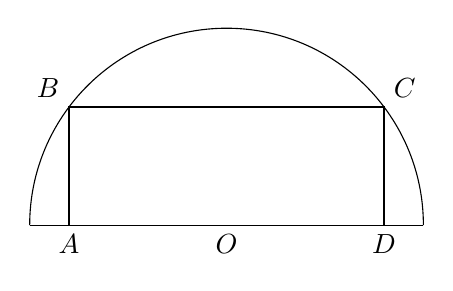
\begin{tikzpicture}[scale = 0.5, baseline = 0]
					\draw[black] (-5, 0)--(0, 0)--(5, 0) node at (0, 0)[anchor = north] {\(O\)} node at (-4, 0)[anchor = north] {\(A\)} node at (4, 0)[anchor = north] {\(D\)};
					\draw[black] (5, 0) arc[start angle = 0, end angle = 180, radius = 5];
					\draw[black] (-4, 0)--(-4, 3)--(4, 3)--(4, 0) node at (-4, 3)[anchor = south east] {\(B\)} node at (4, 3)[anchor = south west] {\(C\)};  
				\end{tikzpicture}
				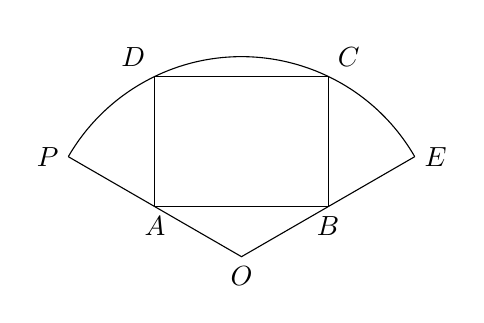
\begin{tikzpicture}[scale = 1.1, baseline = 0]
					\draw[black] (-2, {2 / sqrt(3)})--(0, 0)--(2, {2 / sqrt(3)}) node at (0, 0)[anchor = north] {\(O\)} node at (-1, {1 / sqrt(3)})[anchor = north] {\(A\)} node at (1, {1 / sqrt(3)})[anchor = north] {\(B\)} node at (2, {2 / sqrt(3)})[anchor = west] {\(E\)} node at (-2, {2 / sqrt(3)})[anchor = east] {\(P\)};
					\draw[black] (2, {2 / sqrt(3)}) arc[start angle = 30, end angle = 150, radius = {4 / sqrt(3)}];
					\draw[black] (-1, {1 / sqrt(3)})--(1, {1 / sqrt(3)})--(1, {sqrt(13 / 3)})--(-1, {sqrt(13 / 3)})--(-1, {1 / sqrt(3)}) node at (-1, {sqrt(13 / 3)})[anchor = south east] {\(D\)} node at (1, {sqrt(13 / 3)})[anchor = south west] {\(C\)};
				\end{tikzpicture}
			\]

			\begin{enumerate}[label=\defmath{(\arabic*)}]
				\item 若选定在甲地建设, 求方舱面积的最大值. \answord{\(4 \mathrm{km^2}\)}

					\answord{解析. }三角函数的极值性; 三角变换.

					连接\(OB\), 设\(\angle AOB = \theta, \theta \in \left(0, \dfrac{\pi}{2}\right)\). 有\(OB = 2\mathrm{km}, \angle BAO = \dfrac{\pi}{2}\), 显然有\(OA = 2\cos \theta \mathrm{km}, AB = 2\sin \theta \mathrm{km}\), 有

					\begin{align*}
					\ansmath{\max_{\theta \in \left(0, \dfrac{\pi}{2}\right)}S} &= \max_{\theta \in \left(0, \dfrac{\pi}{2}\right)} \left(2 \cdot OA \cdot AB\right)\\
					&= \max_{\theta \in \left(0, \dfrac{\pi}{2}\right)} \left(8 \sin \theta \cos \theta\right) \mathrm{km^2}\\
					&= \max_{\theta \in \left(0, \dfrac{\pi}{2}\right)}(4 \sin 2 \theta) \mathrm{km^2}\\
					&= \at{4 \sin 2 \theta}{\theta = \dfrac{\pi}{4}}\mathrm{km^2}\\
					&\ansmath{= 4 \mathrm{km^2}}.
					\end{align*}

				\item 若选定在乙地建设, 那么为了使乙地方舱的最大面积不小于甲地的, 则至少需要开辟多少长度的半径? \answord{\(2\sqrt[4]{3} \mathrm{km}\).}

					\answord{解析. }三角函数的极值性; 三角变换.

					连接\(OD, OC\), 设\(\angle AOD = \theta, \theta \in \left(0, \dfrac{\pi}{3}\right), OP=OE=r\). 有\(\angle OAD = \dfrac{2\pi}{3}\), 有

					\[
						\frac{r}{\sin\dfrac{2\pi}{3}} = \dfrac{AD}{\sin \theta} - \dfrac{OA}{\sin \left(\dfrac{\pi}{3} - \theta\right)} \Rightarrow AD = \dfrac{2}{\sqrt{3}}r\sin \theta, OA = \dfrac{2}{\sqrt{3}}r\sin \left(\dfrac{\pi}{3} - \theta\right).
					\]

					在\(\triangle AOB\)中有\(OA=OB, \angle AOB = \dfrac{2\pi}{3},\) 有\(\angle OBA = \dfrac{\pi}{6}, AB = \sqrt{3} OA\). 于是有$AB=2r\sin \left(\dfrac{\pi}{3}-\theta\right)$.

					\begin{align*}
						S &= S(r, \theta)\\
						  &= AD \cdot AB\\
						  &= \frac{4}{\sqrt{3}} r^2 \sin\theta \sin\left(\frac{\pi}{3} - \theta\right)\\
						  &= \frac{2}{\sqrt{3}} r^2 \left[\cos \left(2\theta - \frac{\pi}{3}\right) - \cos \frac{\pi}{3}\right]\\
						  &= \frac{2}{\sqrt{3}} r^2 \left[\cos \left(2\theta - \frac{\pi}{3}\right) - \frac{1}{2}\right], r \in (0, +\infty), \theta \in \left(0, \dfrac{\pi}{3}\right).
					\end{align*}

					二元函数\(S=S(r, \theta)\)在定义域内连续且对\(r, \theta\)的偏导数均存在. 下求\(S\)关于\(\theta\)的偏导:

					\begin{align*}
						\frac{\partial S}{\partial \theta} = S_{\theta} =  &= \lim_{\Delta \theta \rightarrow 0}\frac{S(r, \theta + \Delta \theta) - S(r, \theta)}{\Delta \theta}\\
						&= -\frac{4\sqrt{3} r^2 \sin \left(\frac{6\theta - \pi}{3}\right)}{3}.
					\end{align*}

					考虑\(\dfrac{\partial S}{\partial \theta} = 0\), 有$\theta = \dfrac{\pi}{6}$, 且对\(\theta \in \left(0, \dfrac{\pi}{6}\right): \dfrac{\partial S}{\partial \theta}>0, \)对\(\theta \in \left(\dfrac{\pi}{6}, \dfrac{\pi}{3}\right): \dfrac{\partial S}{\partial \theta}<0\).

					故\(S(r, \theta)\)在\(r\)恒定的时候, 在\(\theta = \dfrac{\pi}{6}\)取到极大值\(\dfrac{1}{\sqrt{3}}r^2 \geq 4 \mathrm{km^2}\). 因此至少开辟\answord{$2\sqrt[4]{3}\mathrm{km}$}.

			\end{enumerate}

	\section{附加题}
		\defword{15. }还没写.

	\section{特别致谢}
		\refword{鸭鸭}, \refword{stOOrz\_OwenXu}, \refword{stOOrz\_BubbleTea }and \refword{Anthan. }提供初版答案参考.

		\refword{stOOrz\_AFOer\_xrh}, \refword{stOOrz\_Jasonying }and \refword{stOOrz\_Jacky\_Chen. }指出预览版中出现的逻辑错误.

\end{document}